\documentclass{beamer}
% Class options include: notes, notesonly, handout, trans,
%                        hidesubsections, shadesubsections,
%                        inrow, blue, red, grey, brown

% Theme for beamer presentation.
\usepackage{beamerthemesplit} 
% Other themes include: beamerthemebars, beamerthemelined, 
%                       beamerthemetree, beamerthemetreebars  

\title[The Practicality of Prompt Engineering]{The Practicality of Prompt Engineering}
\author{Isaac Liu}
\date{\today}

\usepackage{graphicx} % http://ctan.org/pkg/graphicx
\usepackage{amsmath}
\usepackage{geometry}
\usepackage{amsfonts}
\usepackage[english]{babel}
\usepackage{amssymb}
\usepackage{graphicx}
\usepackage{float}
\usepackage{hyperref}
\usepackage{multirow}
\usepackage{pdflscape}
\usepackage{caption}
\usepackage{pdflscape}
\usepackage{outlines}
\usepackage{subcaption}

\usepackage{framed}

\usepackage{tabularx, booktabs}

\usepackage{standalone}

\usepackage[autostyle, english = american]{csquotes}
\MakeOuterQuote{"}

\usepackage{comment}

\hypersetup{
    colorlinks=true,
    linkcolor=white,
    filecolor=black,      
    urlcolor=black,
}

\setbeamertemplate{navigation symbols}{}

\begin{document}

    \begin{frame}
        \frametitle{The Practicality of Prompt Engineering}
        \begin{itemize}
            \item What prompt engineering methods are most effective for a given cost (length/complexity, financial)?
            \item 100 programmatically-conducted conversations
            \item Contribution - quantify with metrics, significance testing, run on new and old models
            \item Statistically Significant Improvements (Paired Tests): GSM8K All, Creative Writing GPT-4 Manual CoT, Zero-Shot CoT
            \item Gains on CW are growing but gains on GSM8K are shrinking in transition from TD3 to GPT-4 % Better with examples in CW, but better to leave to its own on GSM8K
            \item GPT-4 - \$0.03/1K tokens input, \$0.06/1K tokens output
            \item TD3 - \$0.02/1K tokens.
        \end{itemize}

        % \begin{figure}[h]
        %     \centering
        %     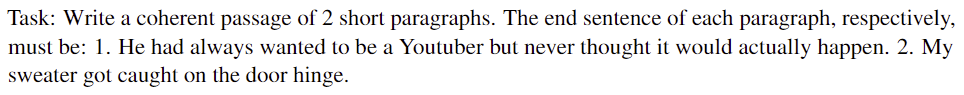
\includegraphics[width=\hsize]{cw_example.png}
        % \end{figure}

        \begin{figure}[h]

            \begin{subfigure}[h]{0.4925\textwidth}
                \centering
                %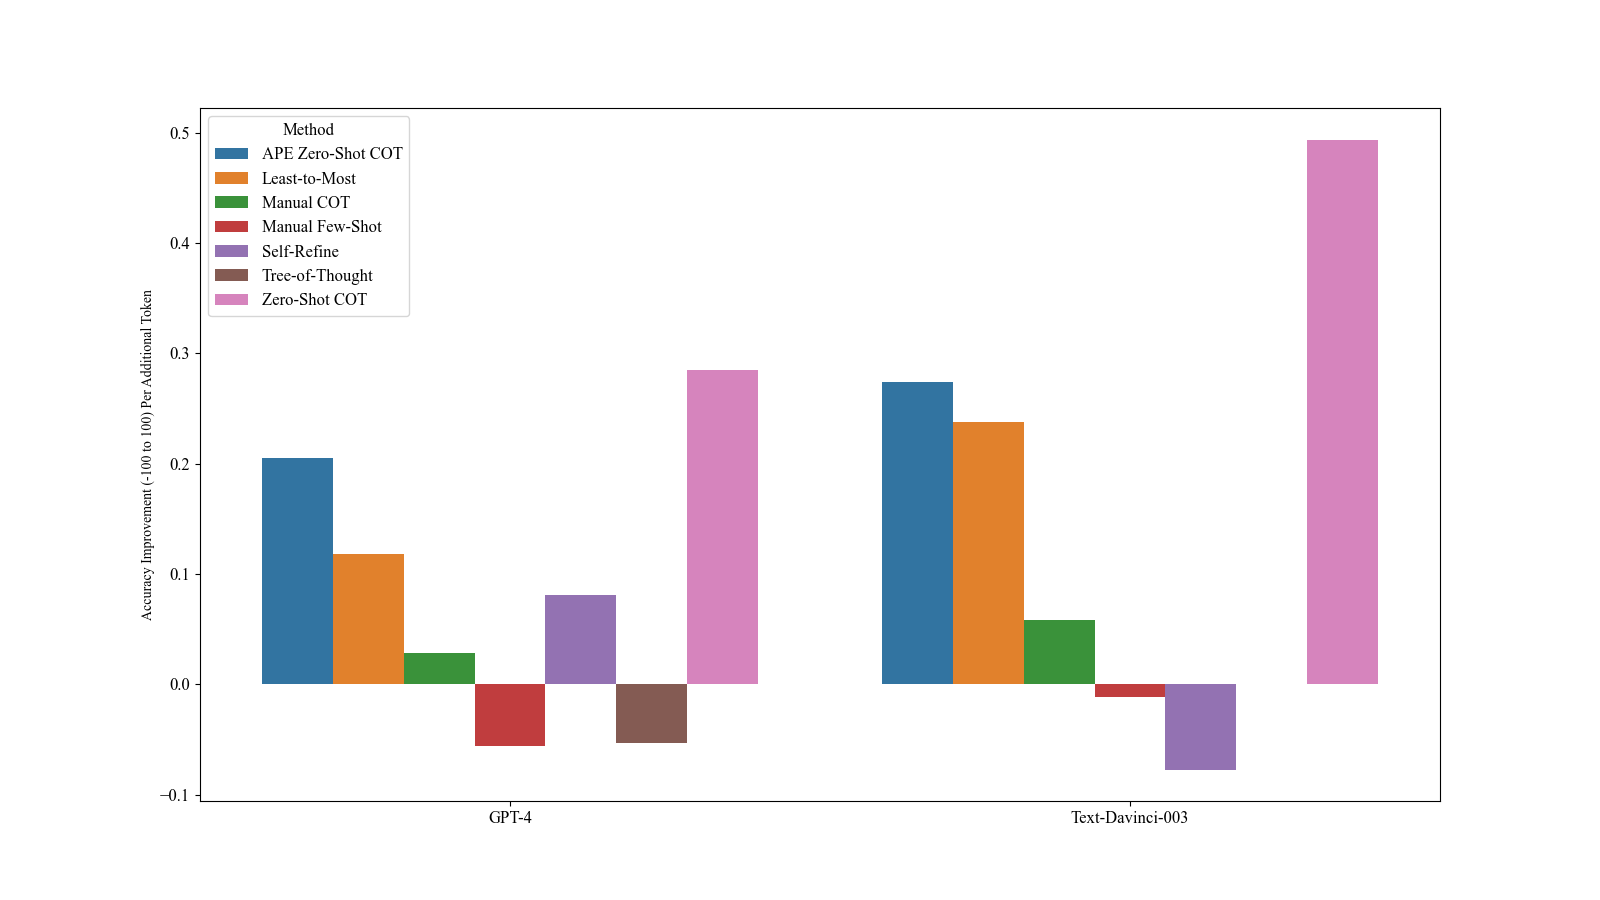
\includegraphics[width=0.95\hsize]{../Output/gsm8k_change_in_accuracy_quality_per_change_in_conversation_length.png} 
                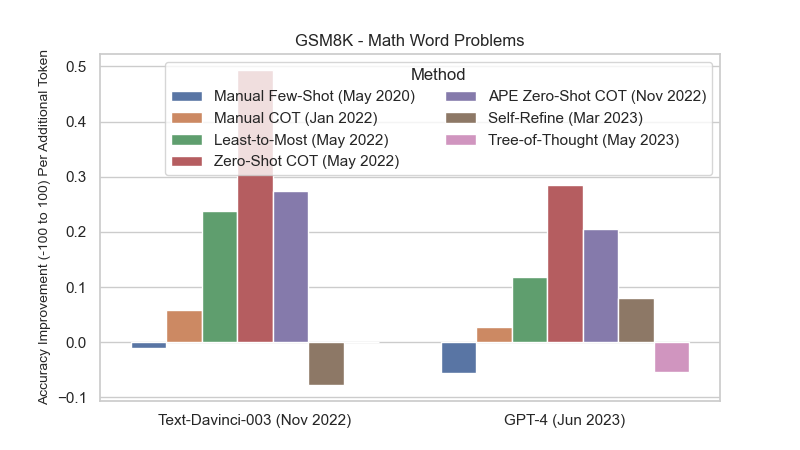
\includegraphics[width=1.1\hsize]{../Output/gsm8k_change_in_accuracy_quality_per_change_in_conversation_length_sorted_by_technique_age.png} 
            \end{subfigure}
            \hfill
            \begin{subfigure}[h]{0.4925\textwidth}
                \centering
                %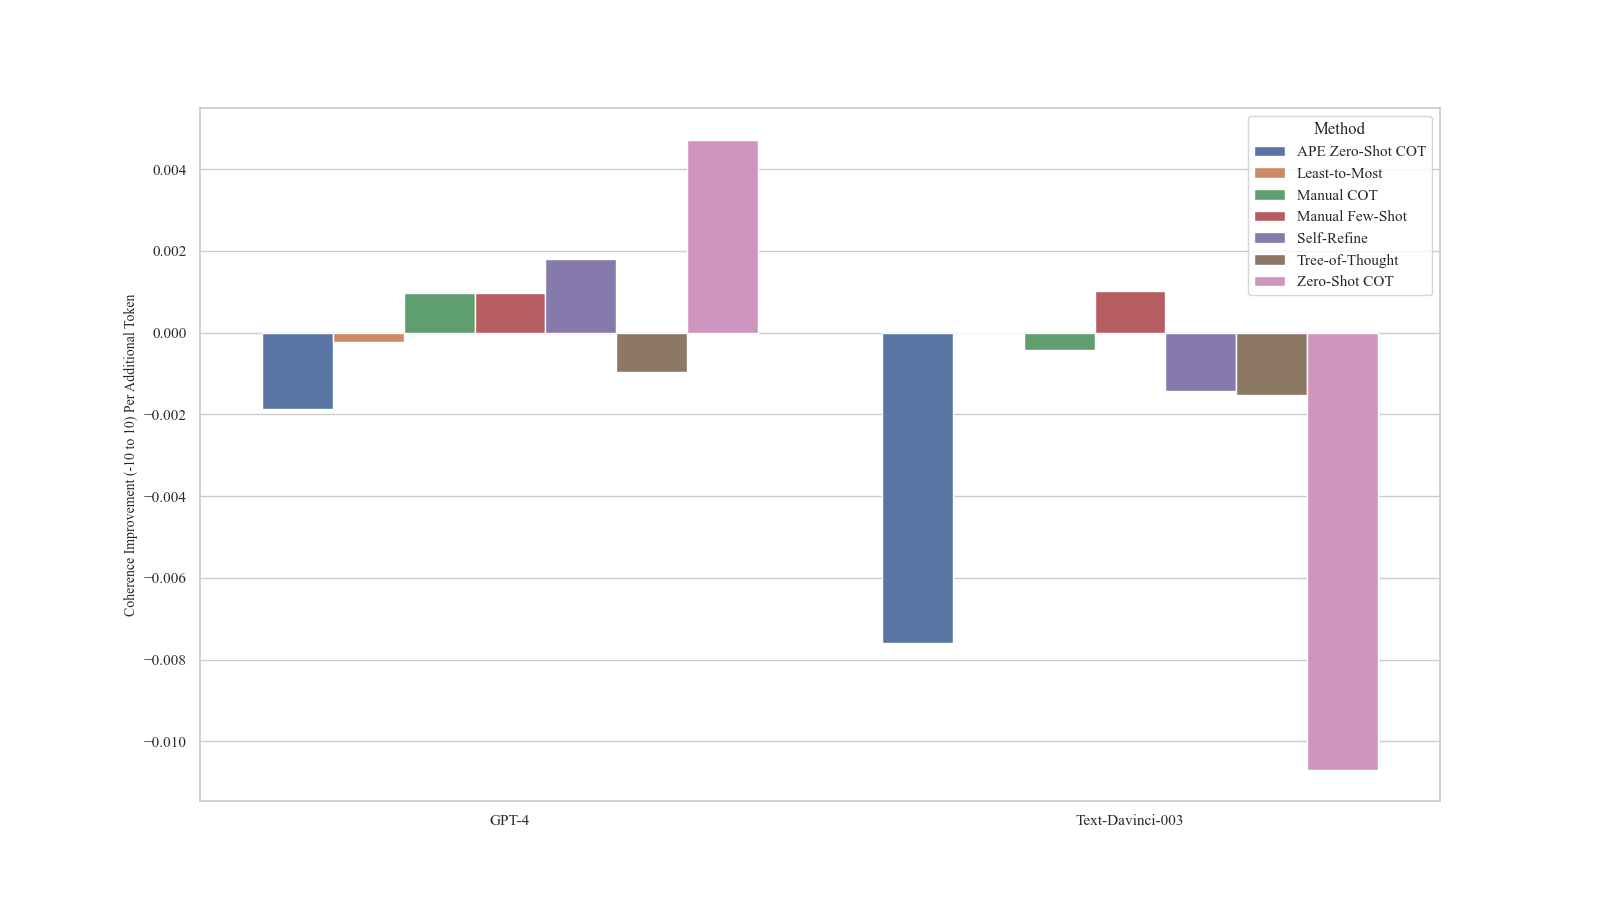
\includegraphics[width=0.95\hsize]{../Output/cw_change_in_accuracy_quality_per_change_in_conversation_length.png}
                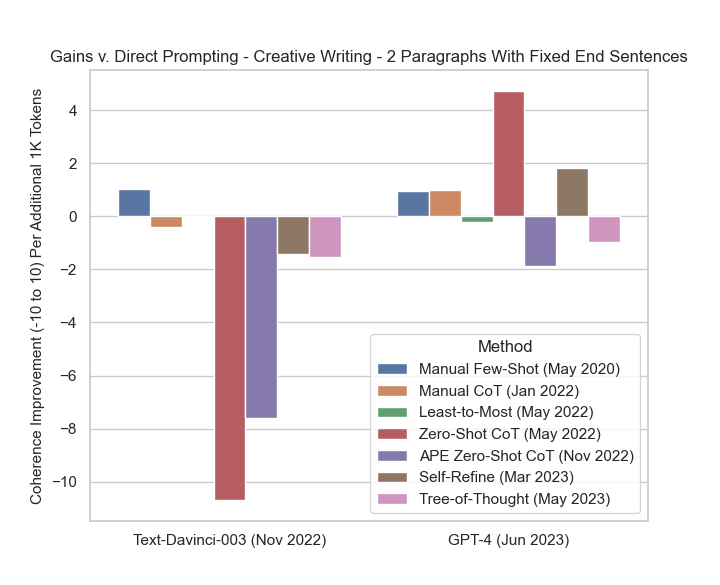
\includegraphics[width=1.1\hsize]{../Output/cw_change_in_accuracy_quality_per_change_in_conversation_length_sorted_by_technique_age_transformed.png}
            \end{subfigure}

        \end{figure}

    \end{frame}

    % \begin{frame}
    %     \frametitle{Theory}
    %     \begin{itemize}
    %         \item Potential theories:
    %         \begin{itemize}
    %             \item Net Welfare Benefits
    %             \begin{itemize}
    %                 \item Inflation time inconsistency problem solved
    %                 \item Increased political efficacy, access to capital
    %             \end{itemize}
    %         \end{itemize}
    %     \end{itemize}

    %     \begin{figure}[h]
    
    %         \begin{subfigure}[h]{0.475\textwidth}
    %             \centering
    %             \includegraphics[width=0.95\hsize]{../../Output/Figures/Fire_JP_Headline.png} 
    %         \end{subfigure}
    %         \hfill
    %         \begin{subfigure}[h]{0.475\textwidth}
    %             \centering
    %             \includegraphics[width=0.95\hsize]{../../Output/Figures/Trump_and_JP.png}
    %         \end{subfigure}
    
    %     \end{figure}

    % \end{frame}

    % \begin{frame}
    %     \frametitle{Ordered Logit Mean Marginal Effects}
    %     {
    %         \let\oldcentering\centering
    %         \renewcommand\centering{\tiny\oldcentering}
    %         \input{../../Output/Tables/ordLogDJ.tex}
    %     }
    % \end{frame}

\end{document}
